\chapter{Implementacija i korisničko sučelje}
		
		
		\section{Korištene tehnologije i alati}
		
			\textbf{\textit{dio 2. revizije}}
			
			 \textit{Detaljno navesti sve tehnologije i alate koji su primijenjeni pri izradi dokumentacije i aplikacije. Ukratko ih opisati, te navesti njihovo značenje i mjesto primjene. Za svaki navedeni alat i tehnologiju je potrebno \textbf{navesti internet poveznicu} gdje se mogu preuzeti ili više saznati o njima}.
			
			
			\eject 
		
	
		\section{Ispitivanje programskog rješenja}
			
			\textbf{\textit{dio 2. revizije}}\\
			
			 \textit{U ovom poglavlju je potrebno opisati provedbu ispitivanja implementiranih funkcionalnosti na razini komponenti i na razini cijelog sustava s prikazom odabranih ispitnih slučajeva. Studenti trebaju ispitati temeljnu funkcionalnost i rubne uvjete.}
	
			
			\subsection{Ispitivanje komponenti}
			\textit{Potrebno je provesti ispitivanje jedinica (engl. unit testing) nad razredima koji implementiraju temeljne funkcionalnosti. Razraditi \textbf{minimalno 6 ispitnih slučajeva} u kojima će se ispitati redovni slučajevi, rubni uvjeti te izazivanje pogreške (engl. exception throwing). Poželjno je stvoriti i ispitni slučaj koji koristi funkcionalnosti koje nisu implementirane. Potrebno je priložiti izvorni kôd svih ispitnih slučajeva te prikaz rezultata izvođenja ispita u razvojnom okruženju (prolaz/pad ispita). }
			
			
			
			\subsection{Ispitivanje sustava}
			
			 \textit{Potrebno je provesti i opisati ispitivanje sustava koristeći radni okvir Selenium\footnote{\url{https://www.seleniumhq.org/}}. Razraditi \textbf{minimalno 4 ispitna slučaja} u kojima će se ispitati redovni slučajevi, rubni uvjeti te poziv funkcionalnosti koja nije implementirana/izaziva pogrešku kako bi se vidjelo na koji način sustav reagira kada nešto nije u potpunosti ostvareno. Ispitni slučaj se treba sastojati od ulaza (npr. korisničko ime i lozinka), očekivanog izlaza ili rezultata, koraka ispitivanja i dobivenog izlaza ili rezultata.\\ }
			 
			 \textit{Izradu ispitnih slučajeva pomoću radnog okvira Selenium moguće je provesti pomoću jednog od sljedeća dva alata:}
			 \begin{itemize}
			 	\item \textit{dodatak za preglednik \textbf{Selenium IDE} - snimanje korisnikovih akcija radi automatskog ponavljanja ispita	}
			 	\item \textit{\textbf{Selenium WebDriver} - podrška za pisanje ispita u jezicima Java, C\#, PHP koristeći posebno programsko sučelje.}
			 \end{itemize}
		 	\textit{Detalji o korištenju alata Selenium bit će prikazani na posebnom predavanju tijekom semestra.}
			
			\eject 
		
		
		\section{Dijagram razmještaja}
			
			\textbf{\textit{dio 2. revizije}}
			
			 \textit{Potrebno je umetnuti \textbf{specifikacijski} dijagram razmještaja i opisati ga. Moguće je umjesto specifikacijskog dijagrama razmještaja umetnuti dijagram razmještaja instanci, pod uvjetom da taj dijagram bolje opisuje neki važniji dio sustava.}
			
			\eject 
		
		\section{Upute za puštanje u pogon}
		
			\indent Puštanje web aplikacije u pogon sastoji se od tri segmenta:
			\begin{itemize}
				\item Stvaranje baze podataka
				\item Puštanje backenda u pogon
				\item Puštanje frontenda u pogon
			\end{itemize}
		
			\noindent \textbf{Stvaranje baze podataka}\\
			
			\indent Baza podataka besplatno je spremljena na web-oblaku render.com. Ona se postavlja i osposobljava sljedećim koracima:
			
			\begin{packed_enum}
				\item Stvaranje nove baze
				\begin{itemize}
					\item Za početak je potrebno (nakon registracije na render.com) odabrati opciju \textit{New} te na padajućem izborniku \textit{PostgreSQL}
					\item Pojavljuje se izbornik koji ispunjavamo kao na slici ispod
					\item Biramo \textit{Create Database}
				\end{itemize}
				\begin{figure}[H]
					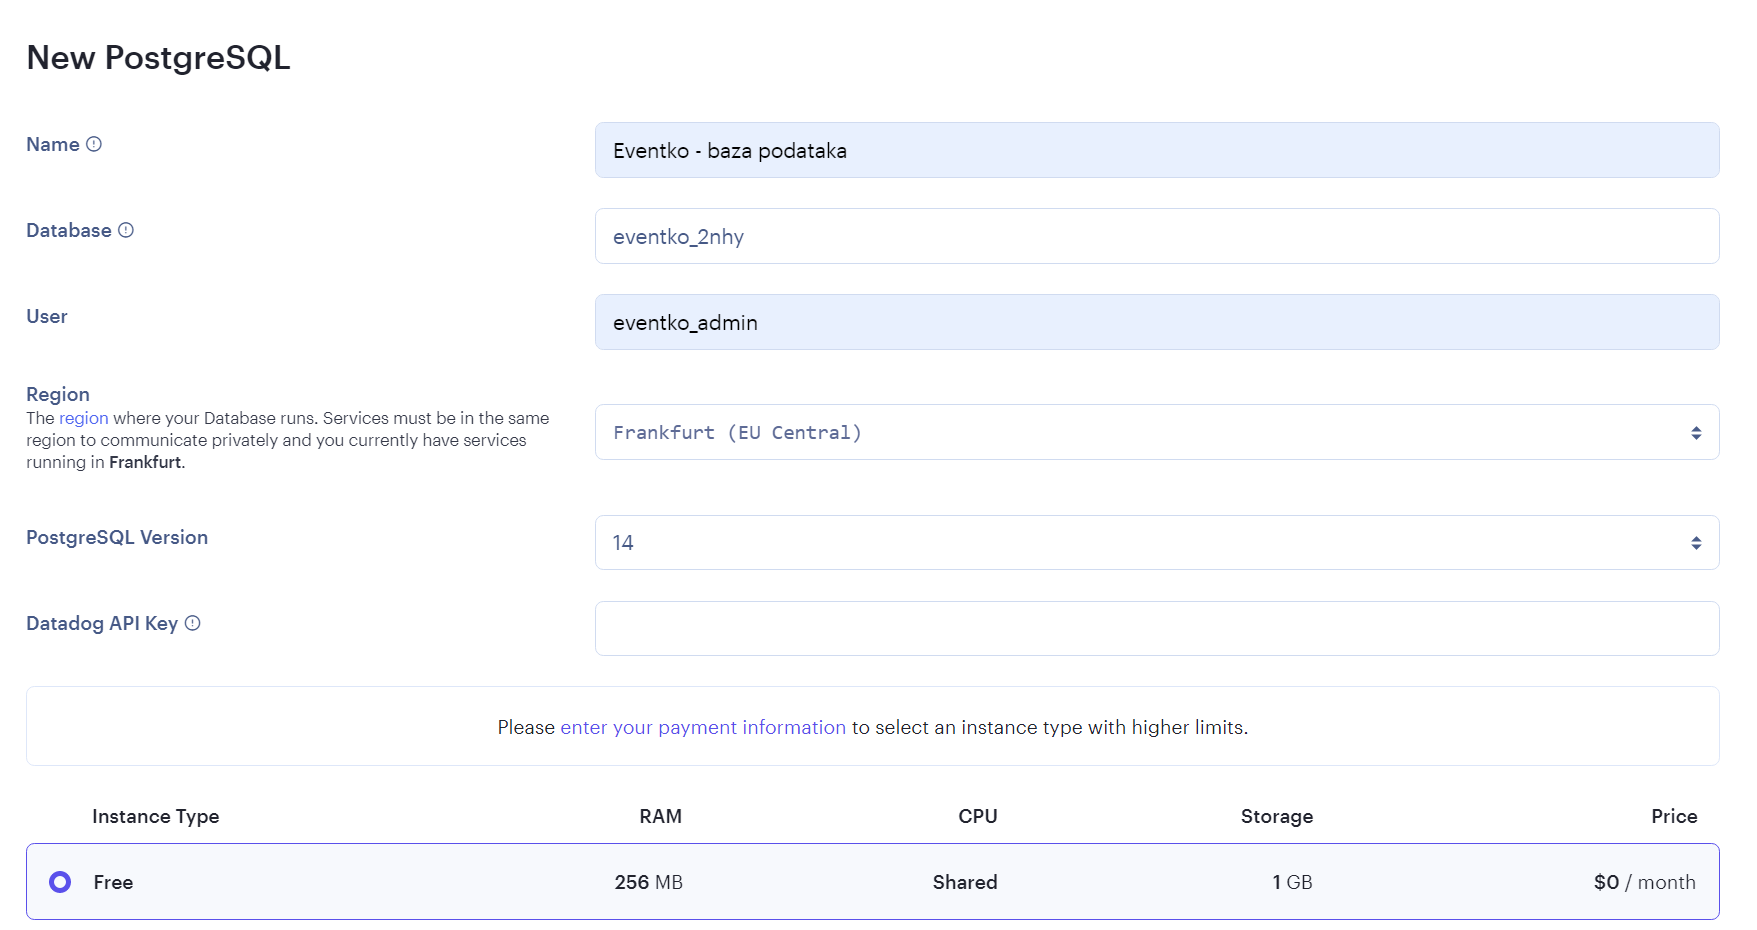
\includegraphics[width=\textwidth]{Opis deploymenta/Slika1.png}
					\caption{Stvaranje nove PostgreSQL baze}
				\end{figure}
				\eject
			
				\item Dohvat podataka za spajanje
				\begin{itemize}
					\item Redom biramo \textit{Dashboard} -> \textit{Eventko - baza podataka} -> \textit{Info}
					\item Skrolamo do izbora \textit{Connections} gdje vidimo informacije potrebne za spajanje na bazu (slika ispod).
				\end{itemize}
				\begin{figure}[H]
					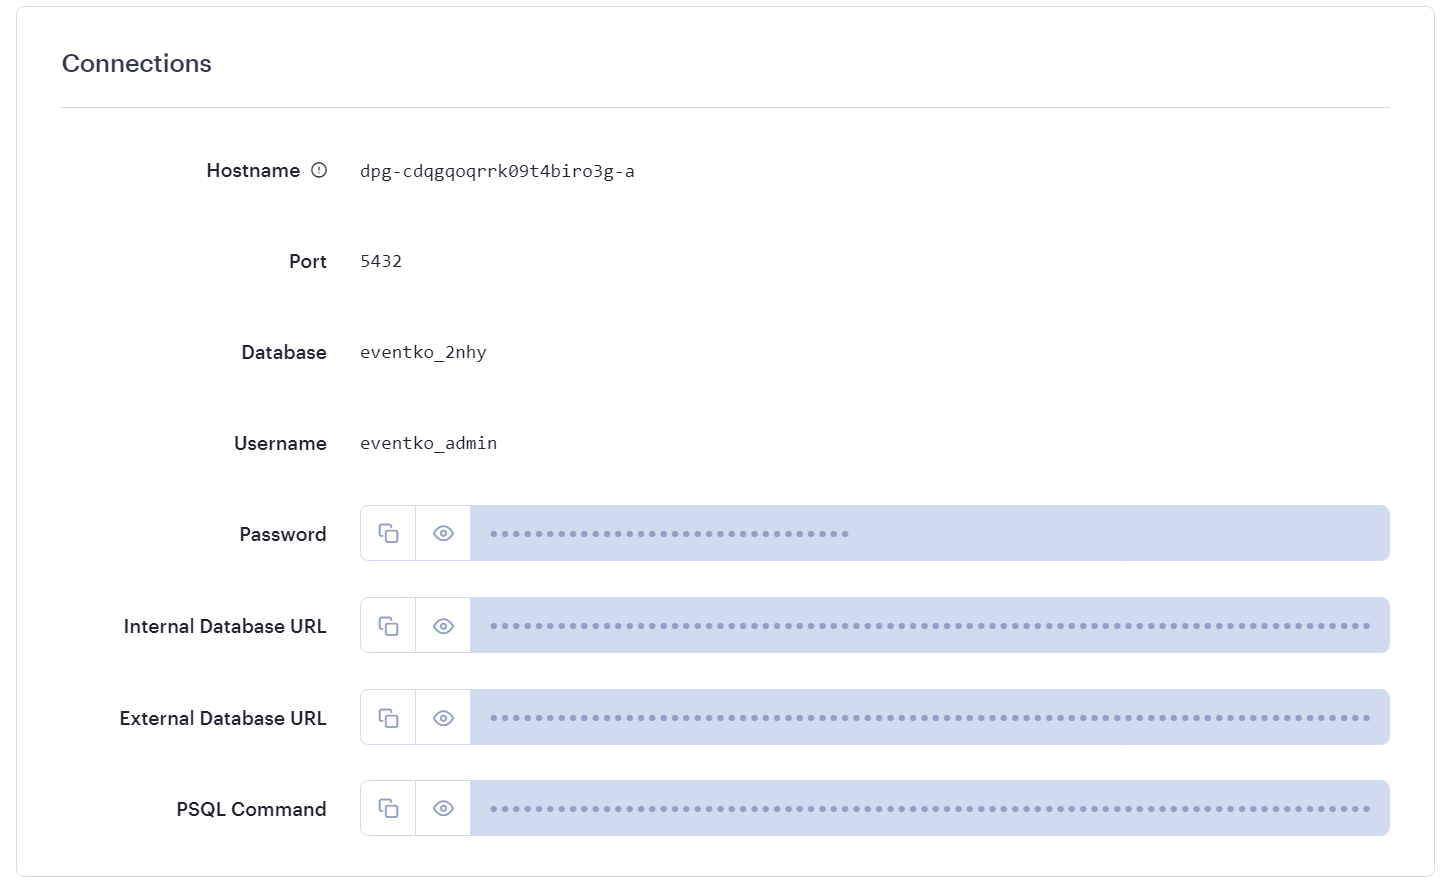
\includegraphics[width=\textwidth]{Opis deploymenta/Slika2.png}
					\caption{Dohvat podataka za spajanje baze}
				\end{figure}
			
				\item Spajanje putem pgAdmina
				\begin{itemize}
					\item Izabiremo \textit{Object} -> \textit{Create} -> \textit{Server}
					\item Na kartici \textit{General} unosimo ime servera kojeg otvaramo u pgAdminu
					\item Na kartici \textit{Connection} unosimo podatke kao na slici i spremamo ih sa \textit{Save}
				\end{itemize}
				\begin{figure}[H]
					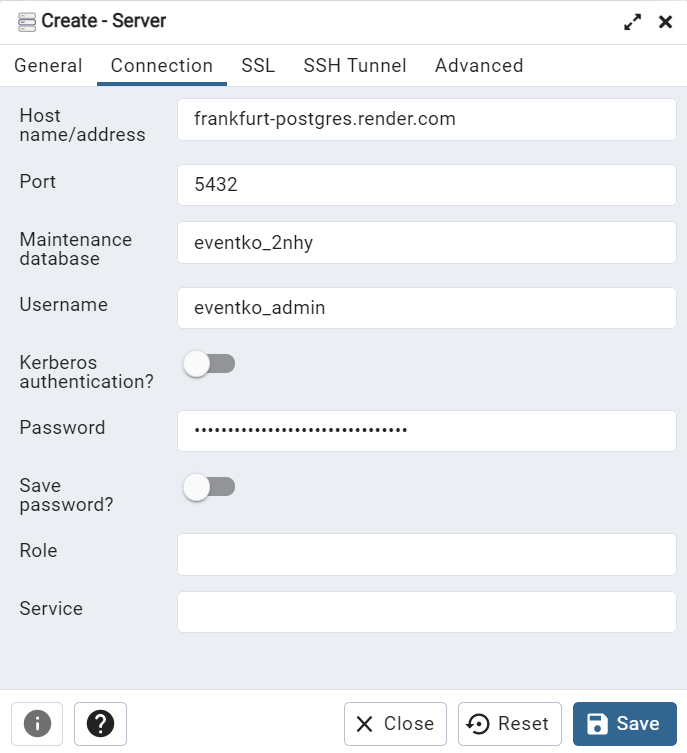
\includegraphics[width=\textwidth]{Opis deploymenta/Slika3.png}
					\caption{Unos podataka za spajanje baze}
				\end{figure}
			
				\item Spajanje iz backenda
				\begin{itemize}
					\item U src/main/resources/application.properties upisujemo naredbe sa slike
				\end{itemize}
				\begin{figure}[H]
					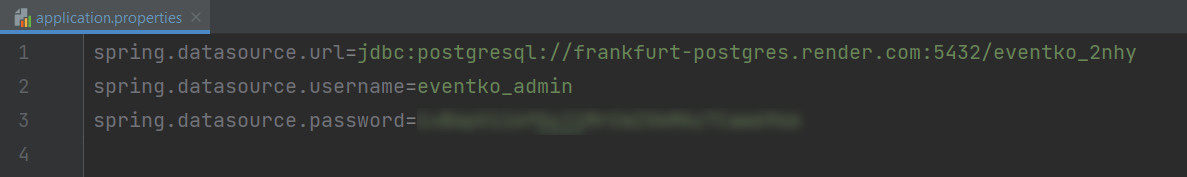
\includegraphics[width=\textwidth]{Opis deploymenta/Slika4.png}
					\caption{Spajanje baze iz backenda}
				\end{figure}
			\end{packed_enum}
			\eject
			
			\noindent \textbf{Puštanje backenda u pogon}\\
			
			\indent Backend dio projekta također koristi render.com za puštanje u pogon. Preduvjeti za to su:		\begin{itemize}
				\item Dodavanje Dockerfilea prikazanog na slici ispod
				\item Povezivanje s GitLabom na renderu
			\end{itemize}
			\begin{figure}[H]
				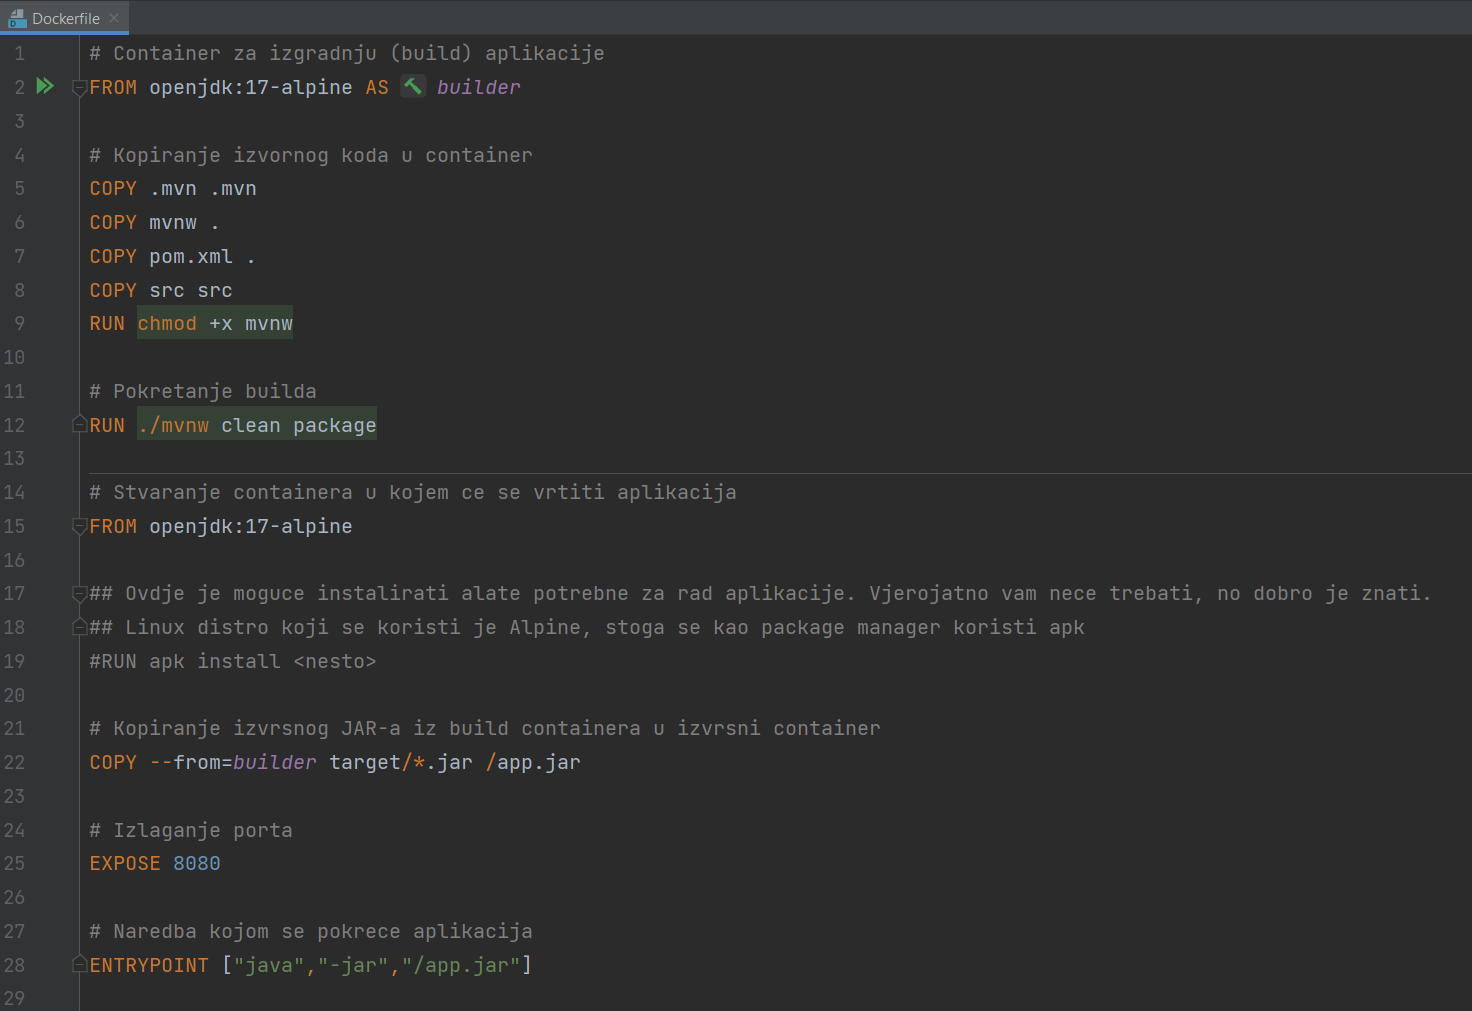
\includegraphics[width=\textwidth]{Opis deploymenta/Slika5.png}
				\caption{Potrebni Dockerfile}
			\end{figure}
		
			\indent Stvaranje backenda postižemo na sljedeći način:
			\begin{itemize}
				\item Odabiremo na render.com \textit{New} -> \textit{Web Service}
				\item Odabiremo željeni GitLab repozitorij
				\item Dalje unosimo podatke kao na slici ispod i potvrđujemo s \textit{Create Web Service}
			\end{itemize}
			\begin{figure}[H]
				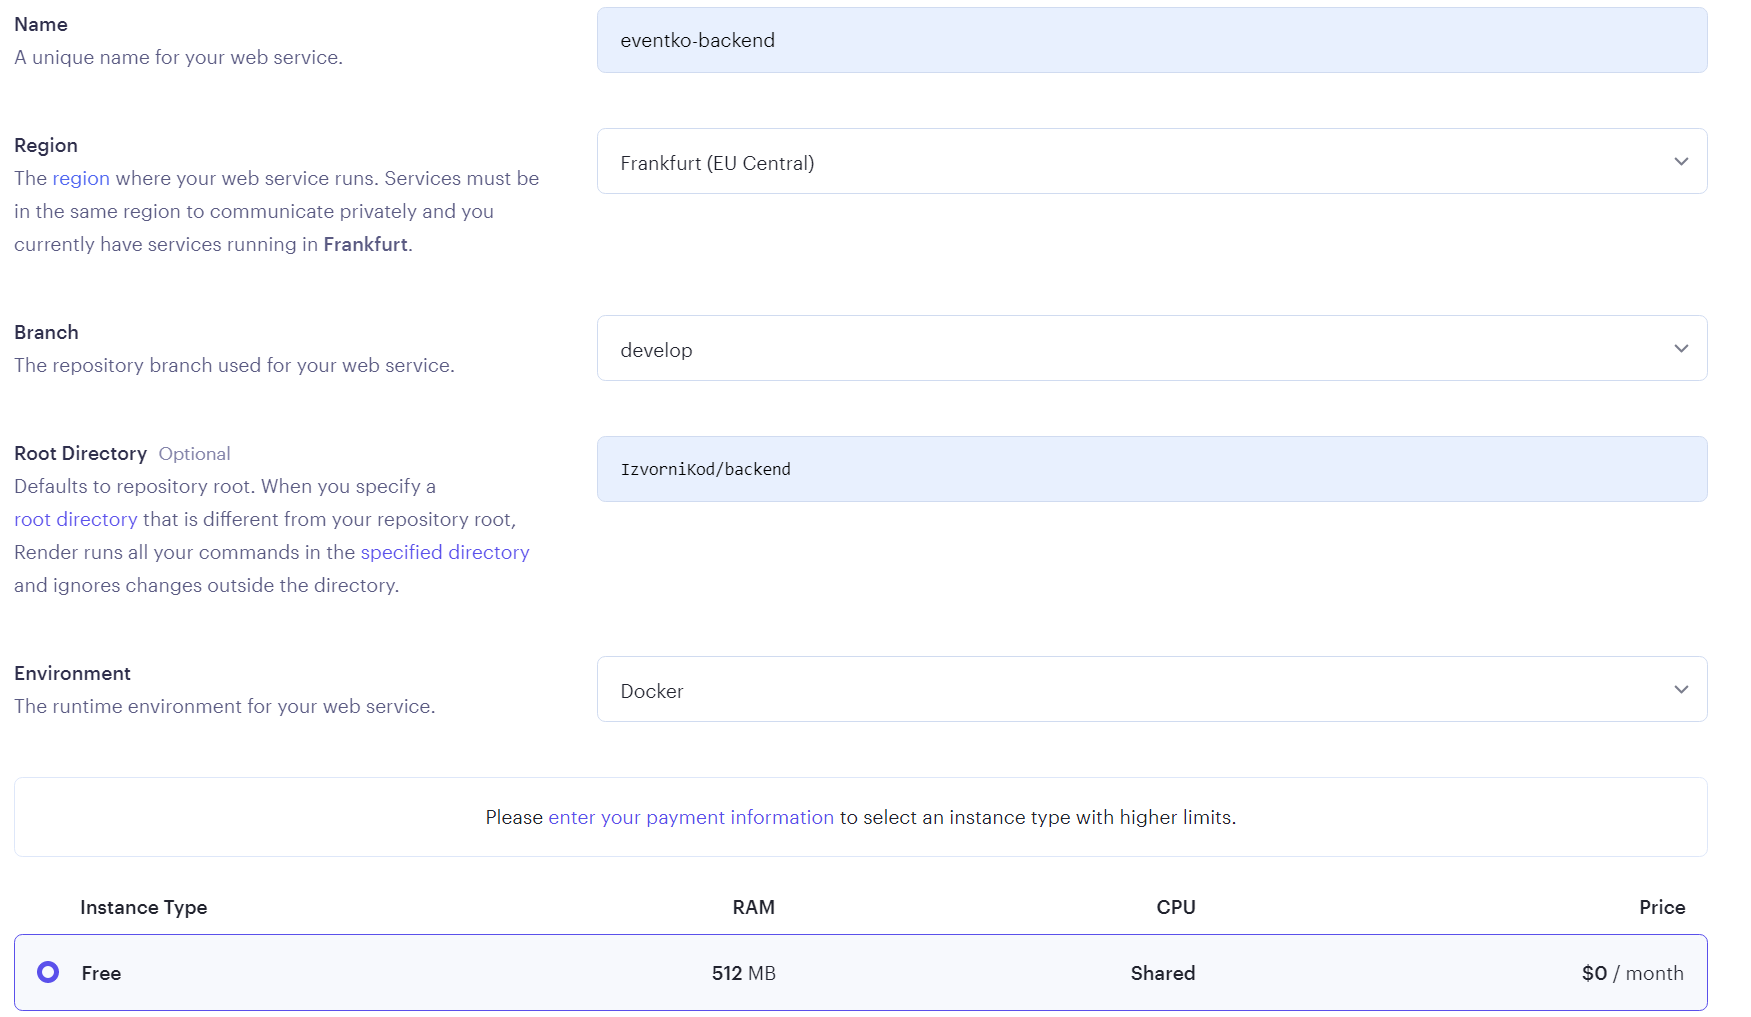
\includegraphics[width=\textwidth]{Opis deploymenta/Slika6.png}
				\caption{Stvaranje novog web servisa}
			\end{figure}
		
			\noindent \textbf{Puštanje frontenda u pogon}\\
			
			\indent Frontend dio projekta puštamo u pogon servisom vercel.com. Preduvjeti za to su:
			\begin{itemize}
				\item Dodavanje vercel.json datoteke u projekt (slika ispod) radi mapiranja putanja prema backendu
				\item Povezivanje s GitLabom i stvaranje grupe na vercelu
			\end{itemize}
		
			\begin{figure}[H]
				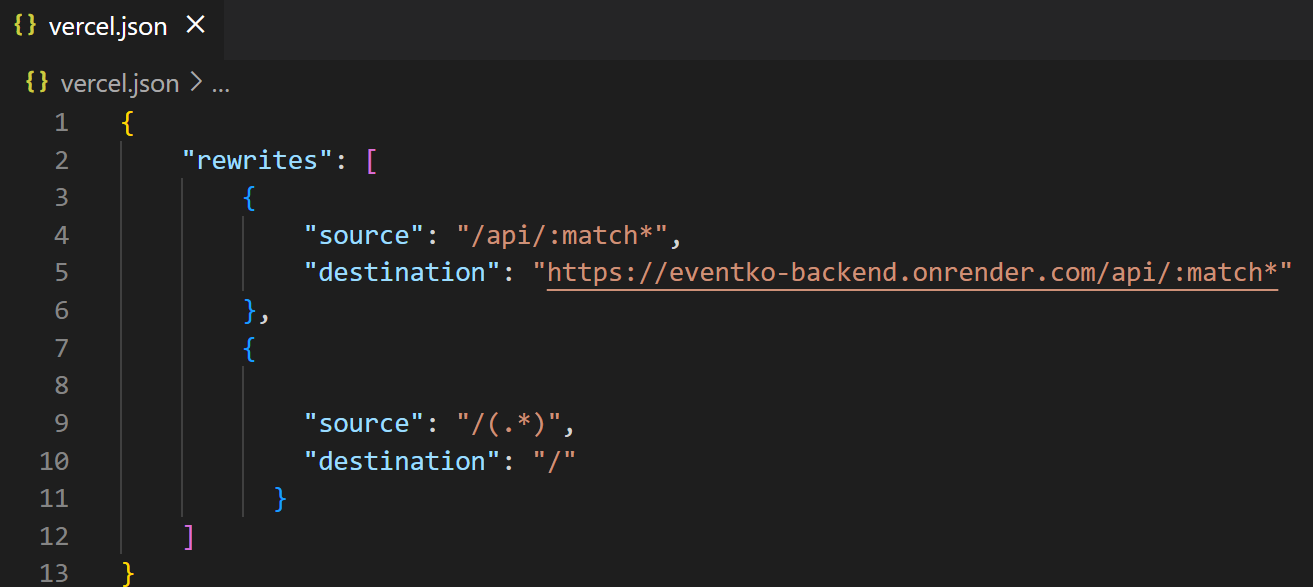
\includegraphics[width=\textwidth]{Opis deploymenta/Slika7.png}
				\caption{Potrebna vercel.json datoteka}
			\end{figure}
			\eject
			
			\indent Za puštanje frontenda u pogon provode se sljedeći koraci:
			\begin{packed_enum}
				\item Stvaranje
				\begin{itemize}
					\item Odabiremo grupu \textit{Vidoje} od ponuđenih iz našeg GitLab računa
					\item Biramo redom \textit{Add new} pa \textit{Import git repository}, pri čemu biramo repozitorij Eventko
					\item Odabiremo \textit{Configure Project}, ispunjavamo polja kao na slici ispod i završavamo s \textit{Deploy}
				\end{itemize}
				\begin{figure}[H]
					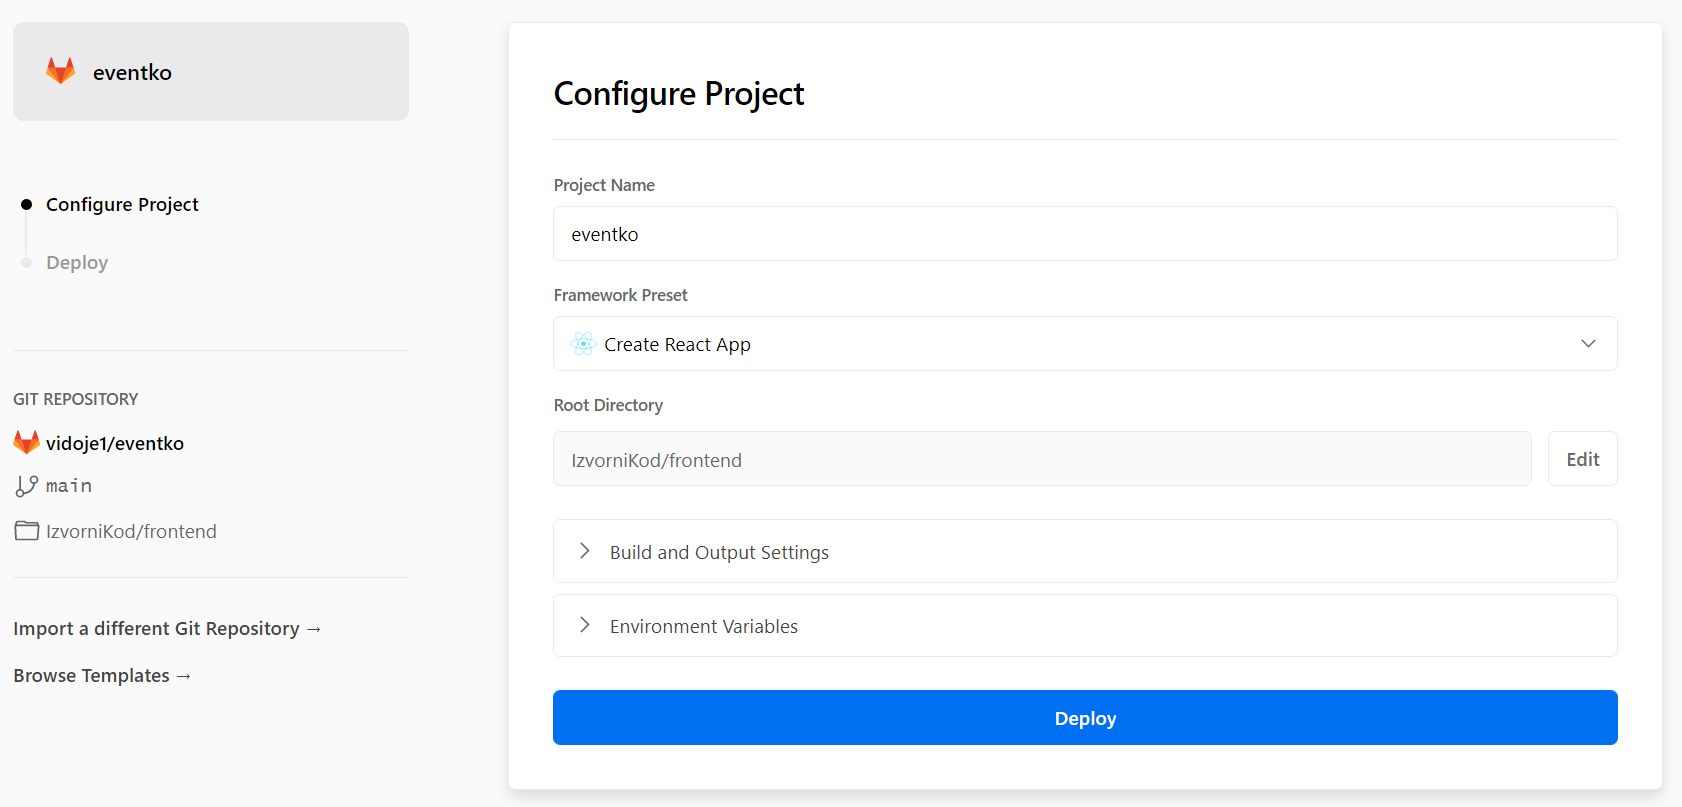
\includegraphics[width=\textwidth]{Opis deploymenta/Slika8.png}
					\caption{Stvaranje React aplikacije i puštanje u pogon}
				\end{figure}
				
				\item Promjena grane
				\begin{itemize}
					\item Biramo redom \textit{Overview} -> \textit{Eventko} -> \textit{Settings} -> \textit{Git}
					\item Mijenjamo granu iz \textit{main} u \textit{develop} kao na slici ispod te spremamo sa \textit{Save}
				\end{itemize}
				\begin{figure}[H]
					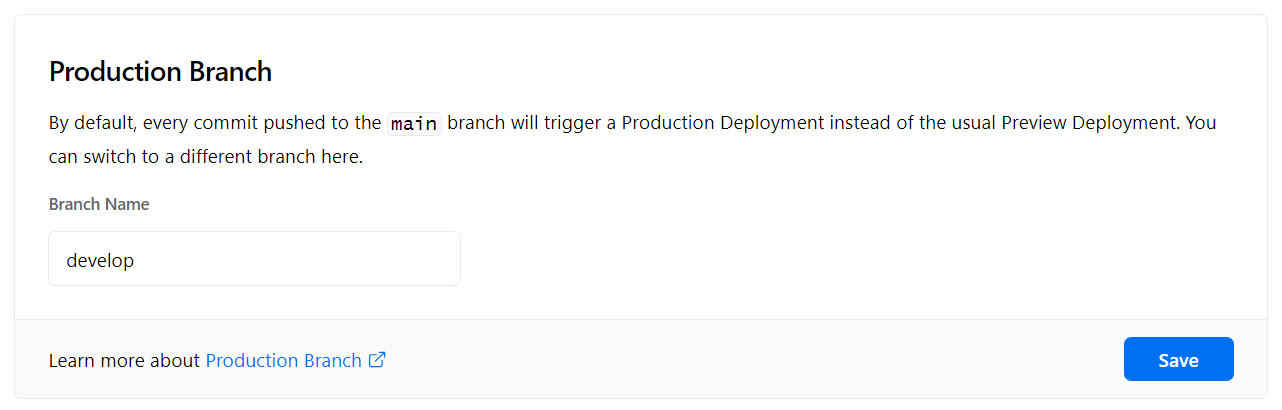
\includegraphics[width=\textwidth]{Opis deploymenta/Slika9.png}
					\caption{Promjena razvojne grane}
				\end{figure}
				\eject
				
				\item Izmjena dodijeljene domene web-stranice (opcionalno)
				\begin{itemize}
					\item Biramo redom \textit{Overview} -> \textit{Eventko} -> \textit{Settings} -> \textit{Domains}
					\item Unosimo novu željenu domenu kao na slici ispod i spremamo sa \textit{Save}
				\end{itemize}
				\begin{figure}[H]
					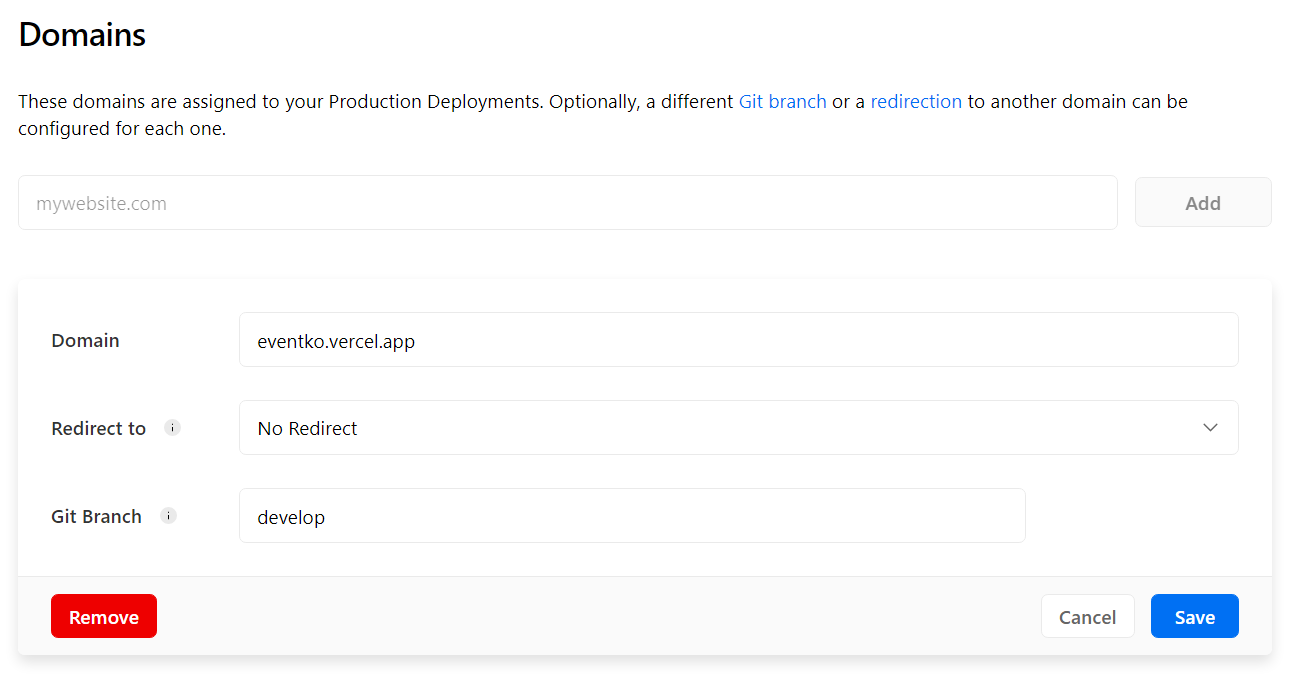
\includegraphics[width=\textwidth]{Opis deploymenta/Slika10.png}
					\caption{Promjena domene web-stranice}
				\end{figure}
			\end{packed_enum}
			
			\eject